
\section{IO-diagram}
Het IO diagram is gebaseerd op de huidige manier van vullen van de dozen.  
\newline
\newline
\begin{figure}[h]
	\centering
	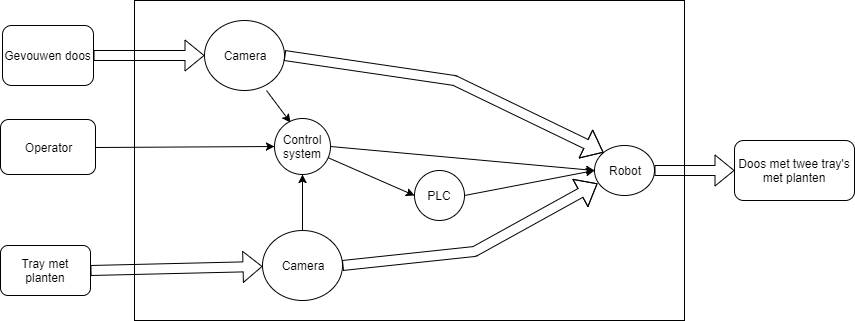
\includegraphics[width=\textwidth]{Afbeeldingen/IO-diagram_v2.png}
	\caption{IO-diagram}
\end{figure}

Aan de invoerkant bevinden zich tray's met planten, een voorgevouwen doos en de input van de operator naar de machine (instelmogelijkheid). De uitkomst is een doos gevuld met twee tray's. \newline
De robot wordt bijgestaan door twee camera's. Een om het oppakken mogelijk te maken en een om de positie en oriëntatie van de doos te vinden. Het control-systeem bindt de componenten aan elkaar en stuurt een PLC aan om de EOAT te bewegen.

%\restoregeometry

\newgeometry{left=3cm, right=3cm, top=3.01cm, bottom=3.01cm} % paperwidth=5.5in, paperheight=8.5in %left=3cm, right=3cm, top=3.01cm, bottom=3.01cm
\pagenumbering{arabic}